%---------------------------------------------------------------------------------------
% Configuracion de Documento
%---------------------------------------------------------------------------------------
\documentclass[10pt, a4paper,english]{article}

\parindent=20pt
\parskip=1pt
\usepackage[width=15.5cm, left=3cm, top=2cm, height= 24.5cm]{geometry}

% User package
\usepackage{epigraph}
\usepackage{amsmath}
\usepackage{amsfonts}
\usepackage{amssymb}
\usepackage{fancyhdr}
\usepackage[activeacute, spanish]{babel}
\usepackage{cancel}
\usepackage[utf8]{inputenc}
%\usepackage{graphicx}
\usepackage{algorithm}
%\usepackage{algorithmic}
%\usepackage{algorithm2e}
\usepackage{algpseudocode}
%\usepackage{afterpage}
\usepackage{lastpage}
\usepackage{listings}
\usepackage{url}
\usepackage{mathptmx}
\usepackage{cite}
\usepackage{pifont}
\usepackage{float}
\usepackage{color}     % para snipets de codigo coloreados
\usepackage{xcolor}
\usepackage{fancybox}  % para el sbox de los snipets de codigo
\usepackage[pdftex]{graphicx}
\usepackage{graphicx} %paquete para incluir imagenes
\usepackage{caption}
\usepackage{subcaption}




\lstset{frame=tb,
	  language=Java,
	  aboveskip=3mm,
	  belowskip=3mm,
	  showstringspaces=false,
	  columns=flexible,
	  basicstyle={\scriptsize\ttfamily},
	  numberstyle=\tiny\color{gray},
	  keywordstyle=\color{blue},
	  commentstyle=\color{green},
	  stringstyle=\color{red},
	  breaklines=true,
	  breakatwhitespace=true,
	  tabsize=3,
	  numbers=left,
	  numbersep=15pt,
	  numberfirstline = false
	}


\pagestyle{fancy}

\thispagestyle{fancy}

\addtolength{\headheight}{1pt}

\lhead{Build a Game-Playing Agent}

\rhead{Leticia L. Rodriguez} % <--- Cambiar de acuerdo al tp actual

\cfoot{\thepage /\pageref{LastPage}}

\renewcommand{\footrulewidth}{0.4pt}

% Informacion del documento

\author{\normalsize{Leticia Lorena Rodr\'iguez}}

\date{\normalsize{February 14th, 2017}} % <--- Cambiar de acuerdo al tp actual

\title{
	
\includegraphics[width=0.05\textwidth]{udacity-small.png}\\
Build a Game-Playing Agent \\
\large {Research Review}
} % <--- Cambiar de acuerdo al tp actual


\begin{document}

\begin{center}


\includegraphics[width=0.05\textwidth]{udacity-small.png}\\
Build a Game-Playing Agent: Heuristic Analysis \\
Leticia L. Rodriguez \\
\end{center}

\section{Introduction}

This summary presents three evaluation functions to winning the Isolation Game.\\ 

Each heuristic idea is evaluated separately and compared to ID\_Improved evaluation function. At the end, a fourth heuristic, combining some of those ideas, is analyzed and presented as final heuristic.\\

\section{Heuristics}

\subsection{Heuristic 1: My moves vs. opponent moves with weight}

\subsubsection{Definition}

The \textit{ID\_Improved} heuristic uses the function:

\[
	score = my\_moves - opponent\_moves
\]

As we saw in the course, this metric could be improved assigning weight to each element. We can define a new evaluation function as:

\[
	score = \textbf{a}*my\_moves + \textbf{b}*opponent\_moves
\]

If $a=1$ and $b=-1$ the new heuristic is equal to ID\_Improved.

It's important to say that some combinations of $a$ and $b$ values are equivalent, for example, $a=1$, $b=-1$ and $a=2$, $b=-2$. 

In order to deal with this issue, in the experimentation section, the values tested are constrained. Further experimentation could go through more values.

Different values of $b$ are analyzed in order to determine new values that achieve better performance than \textit{ID\_Improved}. In particular, the tested function is going to be:

\[
	score = my\_moves \textbf{+} \textbf{b}*opponent\_moves
\]

The score function pseudo-code:\\

\begin{algorithmic}
\Function{MyMovesVsOpponentMoves}{game,player, b}
\If {player looses}
    \State\Return -Inf
\EndIf    
\If {player wins}
   \State \Return +Inf
\Else
	\State myMoves $\leftarrow$ player legal moves
    \State opponentMoves $\leftarrow$ player's opponent legal moves
    \State\Return \#myMoves + b * \#opponentMoves
\EndIf
\EndFunction
\end{algorithmic}

\subsubsection{Experimentation results}

To get accurate results the number of matches for each player (NUM\_MATCHES) has been incremented to 40.   

The idea is to give more weight to those positions with less opponent moves available, so a negative value of \textbf{b}, in range 0 to 6, are going to be used.

The performance rates obtained are shown in this graph:

\begin{center}
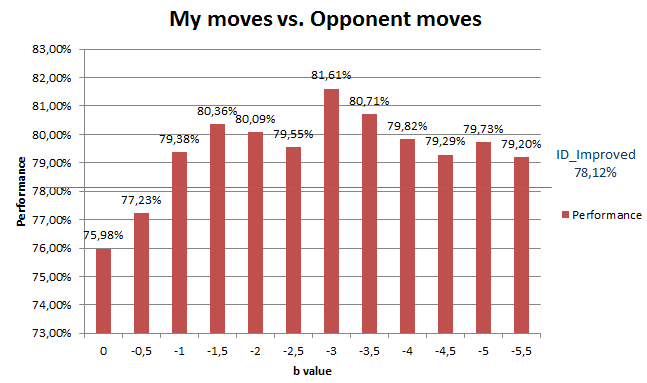
\includegraphics[width=0.8\textwidth]{mymovesopponent.png}\\
\end{center}

For some values, the heuristic beats \textit{ID\_Improved}.

\subsection{Heuristic 2: Center opening}

\subsubsection{Definition}

In Isolation game, the boxes in the center of the board enable more legal moves to the player. \\ 

In the game, the pieces move as knights in chess. The maximum number of moves that a piece could have is 8 moves. \\ 

\begin{center}
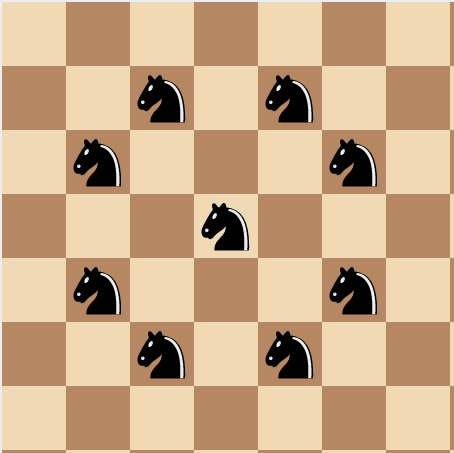
\includegraphics[width=0.3\textwidth]{max_moves.png}\\
\end{center}

In a 7x7 board, the positions with maximum number of moves are: \\

\begin{center}
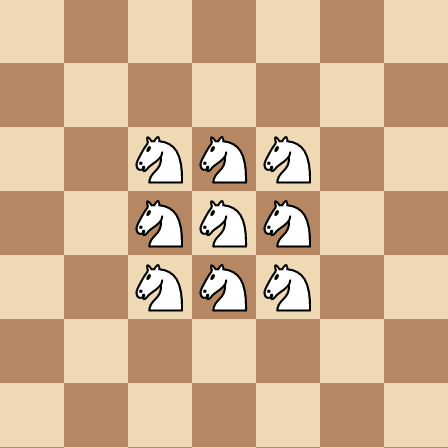
\includegraphics[width=0.3\textwidth]{center_moves.png}\\
\end{center}

The heuristic, proposed in this section, tries to give more weight to moves that put the player in the center of the board. \\

For any board bigger than 5x5 dimension, we can define those center boxes as: \\
\[
(x,y) \;box \; on \; the \; board, \;is\; a\; center\; box\; if\; and\; only\; if\; 2 \leq x < width -2 \;and \; 2 \leq y < height - 2
\]
\\
And the score function pseudo-code:\\

\begin{algorithmic}
\Function{CenterOpening}{game,player, moveCount}
\If {player looses}
    \State\Return -Inf
\EndIf    
\If {player wins}
   \State \Return +Inf
\Else
	\Comment{Game start}
    \State opponentMoves $\leftarrow$ player opponent legal moves
  	\State myMoves $\leftarrow$ player legal moves
    
    \If {game.moves $<$ moveCount}
		\State location $\leftarrow$ player's location on board
        \If{location is a center box}
        	\State\Return 100-\#opponentMoves
        \Else
        	\State\Return \#myMoves -  \#opponentMoves
        \EndIf
    \Else
    	\State\Return \#myMoves -  \#opponentMoves
	\EndIf
\EndIf
\EndFunction
\end{algorithmic}

Notice that the center moves are selected only at the start of the game. The idea is to take advantage of the center of the board at soon as possible in game. Later, the heuristic is going to be similar to ID\_Improved.\\

\subsubsection{Experimentation results}

The algorithm assign a different weight to central positions of the board when the game has recently started. It uses the quantity of moves that have been made in the game to determine whenever apply the center score. \\

Different constraints of moves quantity were tested. The results are:\\

\begin{center}
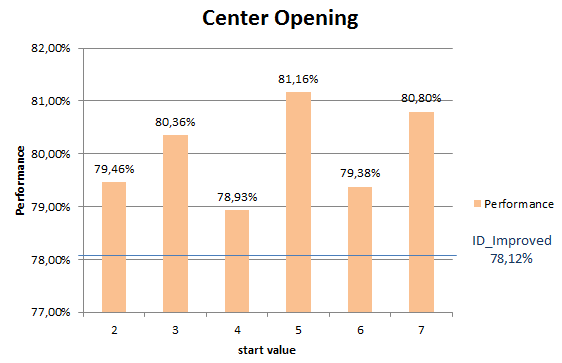
\includegraphics[width=0.7\textwidth]{centeropening.png}\\
\end{center}

Clearly, the graph shows that for all the values tested, the heuristic is better than \textit{ID\_Improved}. Further analysis is needed to determine if there is value where it doesn't occur.

\subsection{Heuristic 3: Common moves}

\subsubsection{Definition}

The player that has no more moves available loose the game. In this evaluation function, the objective is to detect common moves with the opponent in other to grab one of those spots by the current player leaving less options to the opponent.

This heuristic analyze the intersection between my legal moves and my opponent moves and give a higher weight to those nodes with more moves in common.

The computational cost to do an intersection could be high. For the implementation, the \textit{set.intersection} method was used. The selection is based on these results:

\begin{center}
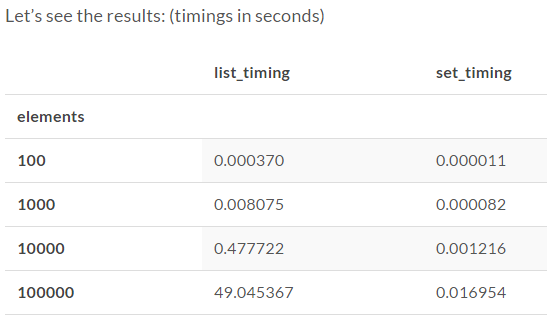
\includegraphics[width=0.5\textwidth]{time_intersec.PNG}\\
\end{center}

{\footnotesize From: http://blog.michelemattioni.me/2015/01/10/list-intersection-in-python-lets-do-it-quickly}/\\

Common moves Heuristic pseudo-code: \\

\begin{algorithmic}
\Function{CommonMoves}{game,player, c}
\If {player looses}
    \State\Return -Inf
\EndIf    
\If {player wins}
   \State \Return +Inf
\Else
		\State myMoves $\leftarrow$ player legal moves
    	\State opponentMoves $\leftarrow$ player's opponent legal moves
        \State commonMoves $\leftarrow$ myMoves $\cap$ opponentMoves
    	\State\Return \#myMoves + \#opponentMoves + c * \#commonMoves
	
\EndIf
\EndFunction
\end{algorithmic}

\subsubsection{Experimentation results}

These are the results of the tests:

\begin{center}
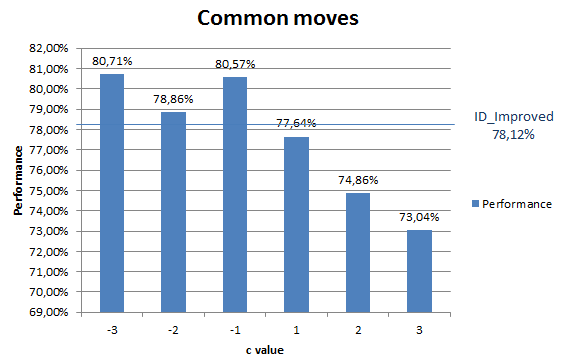
\includegraphics[width=0.7\textwidth]{commonmoves.png}\\
\end{center}

Surprisingly, an improvement against \textit{ID\_Improved} is achieved when common moves has less weight in the score. One explanation could be that the implementation checks player legal moves that are going to be played after the opponent moves, so there is a possibility that opponent select box that are shared with the player. This has the opposite effect than proposed in hypothesis.

\subsection{Final Heuristic: Mixed}

\subsubsection{Definition}

The \textit{ID\_Improved} heuristic has been defeated many times by previous heuristics. In this section, a new evaluation function is introduced base on the combination of best results achieved. \\

In particular, this heuristic is going to be a combination of \textit{Center Opening} and \textit{My Moves vs Opponent Moves with weights}. \\

The starting moves threshold selected for \textit{Center Opening} is going to be fixed in 5 and the opponent moves weight is going to be -3. \\

Proposed Heuristic pseudo-code:\\

\begin{algorithmic}
\Function{FinalHeuristic}{game,player}
\If {player looses}
    \State\Return -Inf
\EndIf    
\If {player wins}
   \State \Return +Inf
\Else
	\Comment{Game start}
    \State opponentMoves $\leftarrow$ player opponent legal moves
  	\State myMoves $\leftarrow$ player legal moves
    
    \If {game.moves $<$ \textbf{5}}
		\State location $\leftarrow$ player location on board
        \If{location is a center box}
        	\State\Return 100-\#opponentMoves
        \Else
        	\State\Return \#myMoves + \textbf{-3} * \#opponentMoves
        \EndIf
    \Else
    	\State\Return \#myMoves + \textbf{-3} * \#opponentMoves
	\EndIf
\EndIf
\EndFunction
\end{algorithmic}


\subsubsection{Experimentation results}

This heuristic was tested against \textit{ID\_Improved} in different NUM\_MATCHES values. The results in this table:\\

\begin{center}
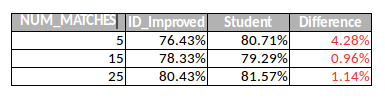
\includegraphics[width=0.7\textwidth]{results.png}\\
\end{center}

\section{Conclusions}

In the present work, three heuristics were introduced:

\begin{itemize}
\item \textbf{My Moves vs Opponent Moves with weights:} that shows better performance than ID\_Improved for some values. 
\item \textbf{Center Opening:} for the values tested it shows always better performance than ID\_Improved.
\item \textbf{Common moves:} that for some values show better performance than ID\_Improved but with an unexpected behavior.
\end{itemize}

Finally, it combines the two first heuristics with their better results in order to propose a final heuristic.

The recommendation of the mixed heuristic is based on:

\begin{itemize}
  \item It uses an optimization of center opening. So the game start is going to be the same as the evaluate \textit{Center Opening} 
  \item Increase the weight of opponent moves to achieve better results in cases that \textit{Center Opening}  doesn't applies 
  \item The results obtained in experimentation shows a better performance against \textit{ID\_Improved}
\end{itemize}


Due some randomness in execution, besides to have incremented the game match, the new heuristic doesn't seems to have an outstanding result.


% \section{Appendix}

% \subsection{My moves vs opponent moves run results}

% \begin{lstlisting}

% *************************
% Evaluating: Student MyMovesVsOpponent0
% *************************

% Playing Matches:
% ----------
%   Match 1: Student MyMovesVsOpponent0 vs   Random    	Result: 153 to 7
%   Match 2: Student MyMovesVsOpponent0 vs   MM\_Null   	Result: 153 to 7
%   Match 3: Student MyMovesVsOpponent0 vs   MM\_Open   	Result: 124 to 36
%   Match 4: Student MyMovesVsOpponent0 vs MM\_Improved 	Result: 104 to 56
%   Match 5: Student MyMovesVsOpponent0 vs   AB\_Null   	Result: 132 to 28
%   Match 6: Student MyMovesVsOpponent0 vs   AB\_Open   	Result: 95 to 65
%   Match 7: Student MyMovesVsOpponent0 vs AB\_Improved 	Result: 90 to 70


% Results:
% ----------
% Student MyMovesVsOpponent0     75.98%

% *************************
% Evaluating: Student MyMovesVsOpponent0.5
% *************************

% Playing Matches:
% ----------
%   Match 1: Student MyMovesVsOpponent0.5 vs   Random    	Result: 150 to 10
%   Match 2: Student MyMovesVsOpponent0.5 vs   MM\_Null   	Result: 154 to 6
%   Match 3: Student MyMovesVsOpponent0.5 vs   MM\_Open   	Result: 119 to 41
%   Match 4: Student MyMovesVsOpponent0.5 vs MM\_Improved 	Result: 115 to 45
%   Match 5: Student MyMovesVsOpponent0.5 vs   AB\_Null   	Result: 133 to 27
%   Match 6: Student MyMovesVsOpponent0.5 vs   AB\_Open   	Result: 102 to 58
%   Match 7: Student MyMovesVsOpponent0.5 vs AB\_Improved 	Result: 92 to 68


% Results:
% ----------
% Student MyMovesVsOpponent0.5     77.23%

% *************************
% Evaluating: Student MyMovesVsOpponent1
% *************************

% Playing Matches:
% ----------
%   Match 1: Student MyMovesVsOpponent1 vs   Random    	Result: 156 to 4
%   Match 2: Student MyMovesVsOpponent1 vs   MM\_Null   	Result: 147 to 13
%   Match 3: Student MyMovesVsOpponent1 vs   MM\_Open   	Result: 120 to 40
%   Match 4: Student MyMovesVsOpponent1 vs MM\_Improved 	Result: 110 to 50
%   Match 5: Student MyMovesVsOpponent1 vs   AB\_Null   	Result: 140 to 20
%   Match 6: Student MyMovesVsOpponent1 vs   AB\_Open   	Result: 115 to 45
%   Match 7: Student MyMovesVsOpponent1 vs AB\_Improved 	Result: 101 to 59


% Results:
% ----------
% Student MyMovesVsOpponent1     79.38%

% *************************
% Evaluating: Student MyMovesVsOpponent1.5
% *************************

% Playing Matches:
% ----------
%   Match 1: Student MyMovesVsOpponent1.5 vs   Random    	Result: 157 to 3
%   Match 2: Student MyMovesVsOpponent1.5 vs   MM\_Null   	Result: 156 to 4
%   Match 3: Student MyMovesVsOpponent1.5 vs   MM\_Open   	Result: 127 to 33
%   Match 4: Student MyMovesVsOpponent1.5 vs MM\_Improved 	Result: 115 to 45
%   Match 5: Student MyMovesVsOpponent1.5 vs   AB\_Null   	Result: 141 to 19
%   Match 6: Student MyMovesVsOpponent1.5 vs   AB\_Open   	Result: 106 to 54
%   Match 7: Student MyMovesVsOpponent1.5 vs AB\_Improved 	Result: 98 to 62


% Results:
% ----------
% Student MyMovesVsOpponent1.5     80.36%

% *************************
% Evaluating: Student MyMovesVsOpponent2
% *************************

% Playing Matches:
% ----------
%   Match 1: Student MyMovesVsOpponent2 vs   Random    	Result: 158 to 2
%   Match 2: Student MyMovesVsOpponent2 vs   MM\_Null   	Result: 154 to 6
%   Match 3: Student MyMovesVsOpponent2 vs   MM\_Open   	Result: 120 to 40
%   Match 4: Student MyMovesVsOpponent2 vs MM\_Improved 	Result: 115 to 45
%   Match 5: Student MyMovesVsOpponent2 vs   AB\_Null   	Result: 134 to 26
%   Match 6: Student MyMovesVsOpponent2 vs   AB\_Open   	Result: 116 to 44
%   Match 7: Student MyMovesVsOpponent2 vs AB\_Improved 	Result: 100 to 60


% Results:
% ----------
% Student MyMovesVsOpponent2     80.09%

% *************************
% Evaluating: Student MyMovesVsOpponent2.5
% *************************

% Playing Matches:
% ----------
%   Match 1: Student MyMovesVsOpponent2.5 vs   Random    	Result: 156 to 4
%   Match 2: Student MyMovesVsOpponent2.5 vs   MM\_Null   	Result: 146 to 14
%   Match 3: Student MyMovesVsOpponent2.5 vs   MM\_Open   	Result: 123 to 37
%   Match 4: Student MyMovesVsOpponent2.5 vs MM\_Improved 	Result: 118 to 42
%   Match 5: Student MyMovesVsOpponent2.5 vs   AB\_Null   	Result: 138 to 22
%   Match 6: Student MyMovesVsOpponent2.5 vs   AB\_Open   	Result: 113 to 47
%   Match 7: Student MyMovesVsOpponent2.5 vs AB\_Improved 	Result: 97 to 63


% Results:
% ----------
% Student MyMovesVsOpponent2.5     79.55%

% *************************
% Evaluating: Student MyMovesVsOpponent3
% *************************

% Playing Matches:
% ----------
%   Match 1: Student MyMovesVsOpponent3 vs   Random    	Result: 147 to 13
%   Match 2: Student MyMovesVsOpponent3 vs   MM\_Null   	Result: 149 to 11
%   Match 3: Student MyMovesVsOpponent3 vs   MM\_Open   	Result: 125 to 35
%   Match 4: Student MyMovesVsOpponent3 vs MM\_Improved 	Result: 125 to 35
%   Match 5: Student MyMovesVsOpponent3 vs   AB\_Null   	Result: 145 to 15
%   Match 6: Student MyMovesVsOpponent3 vs   AB\_Open   	Result: 118 to 42
%   Match 7: Student MyMovesVsOpponent3 vs AB\_Improved 	Result: 105 to 55


% Results:
% ----------
% Student MyMovesVsOpponent3     81.61%

% *************************
% Evaluating: Student MyMovesVsOpponent3.5
% *************************

% Playing Matches:
% ----------
%   Match 1: Student MyMovesVsOpponent3.5 vs   Random    	Result: 154 to 6
%   Match 2: Student MyMovesVsOpponent3.5 vs   MM\_Null   	Result: 153 to 7
%   Match 3: Student MyMovesVsOpponent3.5 vs   MM\_Open   	Result: 125 to 35
%   Match 4: Student MyMovesVsOpponent3.5 vs MM\_Improved 	Result: 120 to 40
%   Match 5: Student MyMovesVsOpponent3.5 vs   AB\_Null   	Result: 145 to 15
%   Match 6: Student MyMovesVsOpponent3.5 vs   AB\_Open   	Result: 108 to 52
%   Match 7: Student MyMovesVsOpponent3.5 vs AB\_Improved 	Result: 99 to 61


% Results:
% ----------
% Student MyMovesVsOpponent3.5     80.71%

% *************************
% Evaluating: Student MyMovesVsOpponent4
% *************************

% Playing Matches:
% ----------
%   Match 1: Student MyMovesVsOpponent4 vs   Random    	Result: 157 to 3
%   Match 2: Student MyMovesVsOpponent4 vs   MM\_Null   	Result: 154 to 6
%   Match 3: Student MyMovesVsOpponent4 vs   MM\_Open   	Result: 129 to 31
%   Match 4: Student MyMovesVsOpponent4 vs MM\_Improved 	Result: 117 to 43
%   Match 5: Student MyMovesVsOpponent4 vs   AB\_Null   	Result: 132 to 28
%   Match 6: Student MyMovesVsOpponent4 vs   AB\_Open   	Result: 112 to 48
%   Match 7: Student MyMovesVsOpponent4 vs AB\_Improved 	Result: 93 to 67


% Results:
% ----------
% Student MyMovesVsOpponent4     79.82%

% *************************
% Evaluating: Student MyMovesVsOpponent4.5
% *************************

% Playing Matches:
% ----------
%   Match 1: Student MyMovesVsOpponent4.5 vs   Random    	Result: 151 to 9
%   Match 2: Student MyMovesVsOpponent4.5 vs   MM\_Null   	Result: 147 to 13
%   Match 3: Student MyMovesVsOpponent4.5 vs   MM\_Open   	Result: 124 to 36
%   Match 4: Student MyMovesVsOpponent4.5 vs MM\_Improved 	Result: 115 to 45
%   Match 5: Student MyMovesVsOpponent4.5 vs   AB\_Null   	Result: 142 to 18
%   Match 6: Student MyMovesVsOpponent4.5 vs   AB\_Open   	Result: 111 to 49
%   Match 7: Student MyMovesVsOpponent4.5 vs AB\_Improved 	Result: 98 to 62


% Results:
% ----------
% Student MyMovesVsOpponent4.5     79.29%

% *************************
% Evaluating: Student MyMovesVsOpponent5
% *************************

% Playing Matches:
% ----------
%   Match 1: Student MyMovesVsOpponent5 vs   Random    	Result: 155 to 5
%   Match 2: Student MyMovesVsOpponent5 vs   MM\_Null   	Result: 150 to 10
%   Match 3: Student MyMovesVsOpponent5 vs   MM\_Open   	Result: 118 to 42
%   Match 4: Student MyMovesVsOpponent5 vs MM\_Improved 	Result: 123 to 37
%   Match 5: Student MyMovesVsOpponent5 vs   AB\_Null   	Result: 136 to 24
%   Match 6: Student MyMovesVsOpponent5 vs   AB\_Open   	Result: 107 to 53
%   Match 7: Student MyMovesVsOpponent5 vs AB\_Improved 	Result: 104 to 56


% Results:
% ----------
% Student MyMovesVsOpponent5     79.73%

% *************************
% Evaluating: Student MyMovesVsOpponent5.5
% *************************

% Playing Matches:
% ----------
%   Match 1: Student MyMovesVsOpponent5.5 vs   Random    	Result: 156 to 4
%   Match 2: Student MyMovesVsOpponent5.5 vs   MM\_Null   	Result: 147 to 13
%   Match 3: Student MyMovesVsOpponent5.5 vs   MM\_Open   	Result: 122 to 38
%   Match 4: Student MyMovesVsOpponent5.5 vs MM\_Improved 	Result: 119 to 41
%   Match 5: Student MyMovesVsOpponent5.5 vs   AB\_Null   	Result: 140 to 20
%   Match 6: Student MyMovesVsOpponent5.5 vs   AB\_Open   	Result: 107 to 53
%   Match 7: Student MyMovesVsOpponent5.5 vs AB\_Improved 	Result: 96 to 64


% Results:
% ----------
% Student MyMovesVsOpponent5.5     79.20%
% \end{lstlisting}


% \subsection{Center Opening}
% \begin{lstlisting}
% *************************
% Evaluating: Student GameStart
% *************************

% Playing Matches:
% ----------
%   Match 1: Student GameStart vs   Random    	Result: 155 to 5
%   Match 2: Student GameStart vs   MM_Null   	Result: 145 to 15
%   Match 3: Student GameStart vs   MM_Open   	Result: 130 to 30
%   Match 4: Student GameStart vs MM_Improved 	Result: 123 to 37
%   Match 5: Student GameStart vs   AB_Null   	Result: 134 to 26
%   Match 6: Student GameStart vs   AB_Open   	Result: 102 to 58
%   Match 7: Student GameStart vs AB_Improved 	Result: 101 to 59


% Results:
% ----------
% Student GameStart  2   79.46%

% *************************
% Evaluating: Student GameStart
% *************************

% Playing Matches:
% ----------
%   Match 1: Student GameStart vs   Random    	Result: 158 to 2
%   Match 2: Student GameStart vs   MM_Null   	Result: 148 to 12
%   Match 3: Student GameStart vs   MM_Open   	Result: 124 to 36
%   Match 4: Student GameStart vs MM_Improved 	Result: 116 to 44
%   Match 5: Student GameStart vs   AB_Null   	Result: 144 to 16
%   Match 6: Student GameStart vs   AB_Open   	Result: 107 to 53
%   Match 7: Student GameStart vs AB_Improved 	Result: 103 to 57


% Results:
% ----------
% Student GameStart  3   80.36%

% *************************
% Evaluating: Student GameStart
% *************************

% Playing Matches:
% ----------
%   Match 1: Student GameStart vs   Random    	Result: 154 to 6
%   Match 2: Student GameStart vs   MM_Null   	Result: 151 to 9
%   Match 3: Student GameStart vs   MM_Open   	Result: 123 to 37
%   Match 4: Student GameStart vs MM_Improved 	Result: 114 to 46
%   Match 5: Student GameStart vs   AB_Null   	Result: 136 to 24
%   Match 6: Student GameStart vs   AB_Open   	Result: 105 to 55
%   Match 7: Student GameStart vs AB_Improved 	Result: 101 to 59


% Results:
% ----------
% Student GameStart  4   78.93%

% *************************
% Evaluating: Student GameStart
% *************************

% Playing Matches:
% ----------
%   Match 1: Student GameStart vs   Random    	Result: 155 to 5
%   Match 2: Student GameStart vs   MM_Null   	Result: 149 to 11
%   Match 3: Student GameStart vs   MM_Open   	Result: 129 to 31
%   Match 4: Student GameStart vs MM_Improved 	Result: 115 to 45
%   Match 5: Student GameStart vs   AB_Null   	Result: 140 to 20
%   Match 6: Student GameStart vs   AB_Open   	Result: 116 to 44
%   Match 7: Student GameStart vs AB_Improved 	Result: 105 to 55


% Results:
% ----------
% Student GameStart   5  81.16%

% *************************
% Evaluating: Student GameStart
% *************************

% Playing Matches:
% ----------
%   Match 1: Student GameStart vs   Random    	Result: 154 to 6
%   Match 2: Student GameStart vs   MM_Null   	Result: 150 to 10
%   Match 3: Student GameStart vs   MM_Open   	Result: 120 to 40
%   Match 4: Student GameStart vs MM_Improved 	Result: 114 to 46
%   Match 5: Student GameStart vs   AB_Null   	Result: 143 to 17
%   Match 6: Student GameStart vs   AB_Open   	Result: 106 to 54
%   Match 7: Student GameStart vs AB_Improved 	Result: 102 to 58


% Results:
% ----------
% Student GameStart  6   79.38%

% *************************
% Evaluating: Student GameStart
% *************************

% Playing Matches:
% ----------
%   Match 1: Student GameStart vs   Random    	Result: 154 to 6
%   Match 2: Student GameStart vs   MM_Null   	Result: 152 to 8
%   Match 3: Student GameStart vs   MM_Open   	Result: 124 to 36
%   Match 4: Student GameStart vs MM_Improved 	Result: 121 to 39
%   Match 5: Student GameStart vs   AB_Null   	Result: 145 to 15
%   Match 6: Student GameStart vs   AB_Open   	Result: 110 to 50
%   Match 7: Student GameStart vs AB_Improved 	Result: 99 to 61


% Results:
% ----------
% Student GameStart    7 80.80%

% Process finished with exit code 0
% \end{lstlisting}

% \subsection{Common Moves}
% \begin{lstlisting}
% *************************
% Evaluating: Student CommonMoves 1
% *************************

% Playing Matches:
% ----------
%   Match 1: Student CommonMoves 1 vs   Random    	Result: 386 to 14
%   Match 2: Student CommonMoves 1 vs   MM_Null   	Result: 366 to 34
%   Match 3: Student CommonMoves 1 vs   MM_Open   	Result: 301 to 99
%   Match 4: Student CommonMoves 1 vs MM_Improved 	Result: 280 to 120
%   Match 5: Student CommonMoves 1 vs   AB_Null   	Result: 332 to 68
%   Match 6: Student CommonMoves 1 vs   AB_Open   	Result: 264 to 136
%   Match 7: Student CommonMoves 1 vs AB_Improved 	Result: 245 to 155


% Results:
% ----------
% Student CommonMoves 1     77.64%

% *************************
% Evaluating: Student CommonMoves 2
% *************************

% Playing Matches:
% ----------
%   Match 1: Student CommonMoves 2 vs   Random    	Result: 384 to 16
%   Match 2: Student CommonMoves 2 vs   MM_Null   	Result: 364 to 36
%   Match 3: Student CommonMoves 2 vs   MM_Open   	Result: 257 to 143
%   Match 4: Student CommonMoves 2 vs MM_Improved 	Result: 259 to 141
%   Match 5: Student CommonMoves 2 vs   AB_Null   	Result: 337 to 63
%   Match 6: Student CommonMoves 2 vs   AB_Open   	Result: 260 to 140
%   Match 7: Student CommonMoves 2 vs AB_Improved 	Result: 235 to 165


% Results:
% ----------
% Student CommonMoves 2     74.86%

% *************************
% Evaluating: Student CommonMoves 3
% *************************

% Playing Matches:
% ----------
%   Match 1: Student CommonMoves 3 vs   Random    	Result: 379 to 21
%   Match 2: Student CommonMoves 3 vs   MM_Null   	Result: 364 to 36
%   Match 3: Student CommonMoves 3 vs   MM_Open   	Result: 261 to 139
%   Match 4: Student CommonMoves 3 vs MM_Improved 	Result: 247 to 153
%   Match 5: Student CommonMoves 3 vs   AB_Null   	Result: 332 to 68
%   Match 6: Student CommonMoves 3 vs   AB_Open   	Result: 239 to 161
%   Match 7: Student CommonMoves 3 vs AB_Improved 	Result: 223 to 177


% Results:
% ----------
% Student CommonMoves 3     73.04%

% Process finished with exit code 0

% *************************
% Evaluating: Student CommonMoves 1
% *************************

% Playing Matches:
% ----------
%   Match 1: Student CommonMoves 1 vs   Random    	Result: 97 to 3
%   Match 2: Student CommonMoves 1 vs   MM_Null   	Result: 98 to 2
%   Match 3: Student CommonMoves 1 vs   MM_Open   	Result: 76 to 24
%   Match 4: Student CommonMoves 1 vs MM_Improved 	Result: 69 to 31
%   Match 5: Student CommonMoves 1 vs   AB_Null   	Result: 88 to 12
%   Match 6: Student CommonMoves 1 vs   AB_Open   	Result: 71 to 29
%   Match 7: Student CommonMoves 1 vs AB_Improved 	Result: 65 to 35


% Results:
% ----------
% Student CommonMoves -1     80.57%

% *************************
% Evaluating: Student CommonMoves 2
% *************************

% Playing Matches:
% ----------
%   Match 1: Student CommonMoves 2 vs   Random    	Result: 94 to 6
%   Match 2: Student CommonMoves 2 vs   MM_Null   	Result: 91 to 9
%   Match 3: Student CommonMoves 2 vs   MM_Open   	Result: 71 to 29
%   Match 4: Student CommonMoves 2 vs MM_Improved 	Result: 74 to 26
%   Match 5: Student CommonMoves 2 vs   AB_Null   	Result: 85 to 15
%   Match 6: Student CommonMoves 2 vs   AB_Open   	Result: 73 to 27
%   Match 7: Student CommonMoves 2 vs AB_Improved 	Result: 64 to 36


% Results:
% ----------
% Student CommonMoves -2     78.86%

% *************************
% Evaluating: Student CommonMoves 3
% *************************

% Playing Matches:
% ----------
%   Match 1: Student CommonMoves 3 vs   Random    	Result: 96 to 4
%   Match 2: Student CommonMoves 3 vs   MM_Null   	Result: 95 to 5
%   Match 3: Student CommonMoves 3 vs   MM_Open   	Result: 78 to 22
%   Match 4: Student CommonMoves 3 vs MM_Improved 	Result: 72 to 28
%   Match 5: Student CommonMoves 3 vs   AB_Null   	Result: 89 to 11
%   Match 6: Student CommonMoves 3 vs   AB_Open   	Result: 71 to 29
%   Match 7: Student CommonMoves 3 vs AB_Improved 	Result: 64 to 36


% Results:
% ----------
% Student CommonMoves -3     80.71%



% \end{lstlisting}


\end{document}
